%\documentclass[12pt,twoside]{article}
\documentclass[conference]{IEEEtran}

%%%%%%% Fill this out:
\newcommand{\trtitle}{Comparison of Neural Architectures \\for Sentiment Analysis of Movie Reviews}
\newcommand{\titleshort}{Sentiment Analysis (Reviews)} % title for header:
\newcommand{\authorlastnames}{Hübner, Pérez} % alphabetical for seminars
\newcommand{\trcourse}{Knowledge Processing in Intelligent Systems: Practical Seminar}
\newcommand{\trgroup}{Knowledge Technology, WTM}
\newcommand{\truniversity}{Department of Informatics, University of Hamburg}
%%%%%%%%%%%%%%%%%%%%%%%%%%%%%%%%%%%%%%%%%%%%%%%%%%%%%%%%%%%%%
% Languages:

% If the thesis is written in English:
\usepackage[english]{babel} 						
\selectlanguage{english}

%%%%%%%%%%%%%%%%%%%%%%%%%%%%%%%%%%%%%%%%%%%%%%%%%%%%%%%%%%%%%
% Bind packages:
\usepackage{lipsum}

\usepackage{acronym}                    % Acronyms
\usepackage{algorithmic}								% Algorithms and Pseudocode
\usepackage{algorithm}									% Algorithms and Pseudocode
\usepackage{amsfonts}                   % AMS Math Packet (Fonts)
\usepackage{amsmath}                    % AMS Math Packet
\usepackage{amssymb}                    % Additional mathematical symbols
\usepackage{amsthm}
\usepackage{booktabs}                   % Nicer tables
%\usepackage[font=small,labelfont=bf]{caption} % Numbered captions for figures
\usepackage{caption} 
\captionsetup[table]{skip=10pt}			% some more space between tables and captions
\usepackage{color}                      % Enables defining of colors via \definecolor
\definecolor{uhhRed}{RGB}{254,0,0}		  % Official Uni Hamburg Red
\definecolor{uhhGrey}{RGB}{122,122,120} % Official Uni Hamburg Grey
\usepackage{fancybox}                   % Gleichungen einrahmen
\usepackage{fancyhdr}										% Packet for nicer headers
%\usepackage{fancyheadings}             % Nicer numbering of headlines

%\usepackage[outer=3.35cm]{geometry} 	  % Type area (size, margins...) !!!Release version
%\usepackage[outer=2.5cm]{geometry} 		% Type area (size, margins...) !!!Print version
%\usepackage{geometry} 									% Type area (size, margins...) !!!Proofread version
\usepackage{geometry} 	  % Type area (size, margins...) !!!Draft version
\geometry{a4paper,body={7.0in,9.1in}}

\usepackage{graphicx}                   % Inclusion of graphics
%\usepackage{latexsym}                  % Special symbols
\usepackage{longtable}									% Allow tables over several parges
\usepackage{listings}                   % Nicer source code listings
\usepackage{multicol}										% Content of a table over several columns
\usepackage{multirow}										% Content of a table over several rows
\usepackage{rotating}										% Alows to rotate text and objects
\usepackage[hang]{subfigure}            % Allows to use multiple (partial) figures in a fig
%\usepackage[font=footnotesize,labelfont=rm]{subfig}	% Pictures in a floating environment
\usepackage{tabularx}										% Tables with fixed width but variable rows
\usepackage{url,xspace,boxedminipage}   % Accurate display of URLs

%%%%%%%%%%%%%%%%%%%%%%%%%%%%%%%%%%%%%%%%%%%%%%%%%%%%%%%%%%%%%
% Configurationen:

\hyphenation{whe-ther} 									% Manually use: "\-" in a word: Staats\-ver\-trag

%\lstloadlanguages{C}                   % Set the default language for listings
\DeclareGraphicsExtensions{.pdf,.svg,.jpg,.png,.eps} % first try pdf, then eps, png and jpg
\graphicspath{{./graphics/}} 								% Path to a folder where all pictures are located
\pagestyle{fancy} 											% Use nicer header and footer

% Redefine the environments for floating objects:
\setcounter{topnumber}{3}
\setcounter{bottomnumber}{2}
\setcounter{totalnumber}{4}
\renewcommand{\topfraction}{0.9} 			  %Standard: 0.7
\renewcommand{\bottomfraction}{0.5}		  %Standard: 0.3
\renewcommand{\textfraction}{0.1}		  	%Standard: 0.2
\renewcommand{\floatpagefraction}{0.8} 	%Standard: 0.5

% Tables with a nicer padding:
\renewcommand{\arraystretch}{1.2}

%%%%%%%%%%%%%%%%%%%%%%%%%%%%
% Additional 'theorem' and 'definition' blocks:
\theoremstyle{plain}
\newtheorem{theorem}{Theorem}[section]
%\newtheorem{theorem}{Satz}[section]		% Wenn in Deutsch geschrieben wird.
\newtheorem{axiom}{Axiom}[section] 	
%\newtheorem{axiom}{Fakt}[chapter]			% Wenn in Deutsch geschrieben wird.
%Usage:%\begin{axiom}[optional description]%Main part%\end{fakt}

\theoremstyle{definition}
\newtheorem{definition}{Definition}[section]

%Additional types of axioms:
\newtheorem{lemma}[axiom]{Lemma}
\newtheorem{observation}[axiom]{Observation}

%Additional types of definitions:
\theoremstyle{remark}
%\newtheorem{remark}[definition]{Bemerkung} % Wenn in Deutsch geschrieben wird.
\newtheorem{remark}[definition]{Remark} 

%%%%%%%%%%%%%%%%%%%%%%%%%%%%
% Provides TODOs within the margin:
\newcommand{\TODO}[1]{\marginpar{\emph{\small{{\bf TODO: } #1}}}}

%%%%%%%%%%%%%%%%%%%%%%%%%%%%
% Abbreviations and mathematical symbols
\newcommand{\modd}{\text{ mod }}
\newcommand{\RS}{\mathbb{R}}
\newcommand{\NS}{\mathbb{N}}
\newcommand{\ZS}{\mathbb{Z}}
\newcommand{\dnormal}{\mathit{N}}
\newcommand{\duniform}{\mathit{U}}

\newcommand{\erdos}{Erd\H{o}s}
\newcommand{\renyi}{-R\'{e}nyi}
\usepackage{graphicx}

%\usepackage{dblfloatfix}	% fix floating figures and tables

% correct bad hyphenation here
\hyphenation{}

%%%%%%%%%%%%%%%%%%%%%%%%%%%%%%%%%%%%%%%%%%%%%%%%%%%%%%%%%%%%%
% Document:
\begin{document}

\title{\trtitle}
\renewcommand{\headheight}{14.5pt}

%\fancyhead{}
%\fancyhead[LE]{  }
\fancyhead[LO]{\slshape \authorlastnames}
%\fancyhead[RE]{}
\fancyhead[RO]{ \slshape \titleshort}

% author names and affiliations
% use a multiple column layout for up to three different
% affiliations
\author{
\IEEEauthorblockN{Sören Hübner\IEEEauthorrefmark{1}, Nicol\'as P\'erez de Olaguer\IEEEauthorrefmark{1}}

\IEEEauthorblockA{
	\{8huebner, 7perez\}@informatik.uni-hamburg.de
}

\medskip

\IEEEauthorblockA{
	\IEEEauthorrefmark{1}\truniversity\\
	\trcourse\\
	\trgroup}
}
%\and 8huebner@informatik.uni-hamburg.de
%\IEEEauthorblockN{Nicol\'as P\'erez de Olaguer}
%\IEEEauthorblockA{7perez@informatik.uni-hamburg.de}
      
% make the title area
\maketitle

\begin{abstract}
	Infering sentiments from text is not always a straightforward procedure. Language systems are usually complex and the use of figures of speech such as irony may lead to wrong conclusions. Several machine learning techniques can be helpful to unveil the underlying complexity of such texts, although prediction accuracy is always an important issue. In this paper, we use the well-known Internet Movie Database (IMDb) data set \cite{imdb_data} and try to predict the sentiment behind a movie review. We compare the performance and applicability of several machine learning approaches including artificial neural networks. This work derives from a Kaggle \cite{Kaggle} competition held in 2016 and is based around our implementation of several different approaches. We used the neural network library keras \cite{keras} for the python programming language \cite{python} to achieve acceptable results with three distinct neural network architectures.
\end{abstract}

\IEEEpeerreviewmaketitle

\section{Introduction}
\label{sec:introduction}

There are several tasks where humans are still better than machines. More specifically, when we talk about human communication and sentiment analysis, algorithms are prone to fail. Since the understanding of communication is not unique and can have several interpretations depending on the sender and the receiver, it can be beneficial to explore how automatic techniques can deal with it. Moreover, the inherent complexity of language makes this even harder. For example, literary nuances such as irony or metaphors increase the difficulty of the classification task.

The goal of this paper is to classify movie reviews into two distinct categories: 'positive' and 'negative'. We use the text of the review, embed it in a certain way and feed the resulting vector into one of three different neural network architectures.

The sentiment mining of expressions or texts is useful for research studies or marketing purposes. In table \ref{tab:rev}, we show an example of two different movie reviews and their corresponding sentiment from the used corpus \cite{imdb_data}. A feature of the IMDb movie reviews is that not all reviews come from cinema experts but from all users of the internet platform. Therefore, reducing manual effort to extract sentiment is useful for the movie industry to know whether a film is well accepted by the general audience based on the reviews. In related work \cite{Pak}, the authors perform sentiment analysis of Tweets with an important distinction between positive, negative and objective statements. Nevertheless, in our case, we do not have the third 'objective' class, because the dataset only includes 'positive' reviews with a given score of 7 or higher (on a scale from 1 to 10) and 'negative' ones with a score of 3 or less. 

\section{Related Work}
\label{sec:rel_work}
First approaches to sentiment and mood mining were relying on basic assumptions. In \cite{Pang} they do a comprehensive review of the more useful techniques for information retrieval.  In \cite{Yang} they infer mood from web blogs using SVM (support vector machine) and CRF (conditional random field) techniques. It is interesting how taking the assumption of relying on the last sentence of the post gives better accuracy for sentiment prediction. 

Since relevance of web blogs has decayed, in \cite{Pak}, they do sentiment analysis for tweets. Again, it is different from our scenario since microblogging can take only up to 140 characters and in our case, we have freedom from the reviewer. However, they reach around 80$\%$ accuracy using a bi-gram model and a Naive Bayes classifier. More novel approaches can be found in \cite{Noguishe} where neural architectures are applied to the same twitter task with an accuracy of 86,4$\%$ using Stanford Twitter Sentiment from Stanford University. It is also worth to mention that the developed tasks proceed from a Kaggle competition \cite{Kaggle}. In that challenge, the top accuracy scores get to 97$\%$ of accuracy. 

\begin{table*}[tbh]
\begin{center}
	\begin{tabular}{ | m{40em} | m{1.5cm}|  } 
		\hline
		\textbf{Review} & \textbf{Sentiment} \\ 
		\hline
		"I dont know why people think this is such a bad movie. Its got a pretty good plot, some good action, and the change of location for Harry does not hurt either. Sure some of its offensive and gratuitous but this is not the only movie like that. Eastwood is in good form as Dirty Harry, and I liked Pat Hingle in this movie as the small town cop. If you liked DIRTY HARRY, then you should see this one, its a lot better than THE DEAD POOL. 4/5" & Positive  \\ 
		\hline
		"I watched this video at a friend's house. I'm glad I did not waste money buying this one. The video cover has a scene from the 1975 movie Capricorn One. The movie starts out with several clips of rocket blow-ups, most not related to manned flight. Sibrel's smoking gun is a short video clip of the astronauts preparing a video broadcast. He edits in his own voice-over instead of letting us listen to what the crew had to say. The video curiously ends with a showing of the Zapruder film. His claims about radiation, shielding, star photography, and others lead me to believe is he extremely ignorant or has some sort of ax to grind against NASA, the astronauts, or American in general. His science is bad, and so is this video." & Negative  \\ 
		\hline
	\end{tabular}
	\caption{Sample of one negative and one positive review from the IMDb dataset.}
	\label{tab:rev}
\end{center}
\end{table*}
\medskip
\section{Background}
\label{sec:background}
\textbf{Artificial neural networks} use linear algebra to 'learn' things, approximate functions, classify data points and do many more things. It consists of several 'neurons' which are grouped into layers which themselves are connected with each other. Those connections are weighted to simulate stronger or softer bonds. Some data vector is given as an input and the network then produces an output vector. This type of architecture has the roots in the brain. The artificial neuron is a mathematical entity that has some weights and an activation function. 

Neuron cells receive connections from other cells and fire when they receive electrical impulses from other connected neurons. It is know, that the more a connection is used, the more stronger it will get. 

A loss or \textbf{cost function} is used to turn the learning aspect of neural networks into an optimization problem. It associates some loss or cost with wrong outputs and 'punishes' a network for performing in an undesirable manner. Usually good answers are reinforced and bad ones are discouraged on the basis of a loss function and a process called 'backpropagation', where the neurons which are more responsible for a certain outcome are encouraged or discouraged the most. Nowadays, artificial neural networks, (ANNs) have been proven to solve a lot of classification and regression problems. 

%\begin{figure}[htb]
%	\centering
%	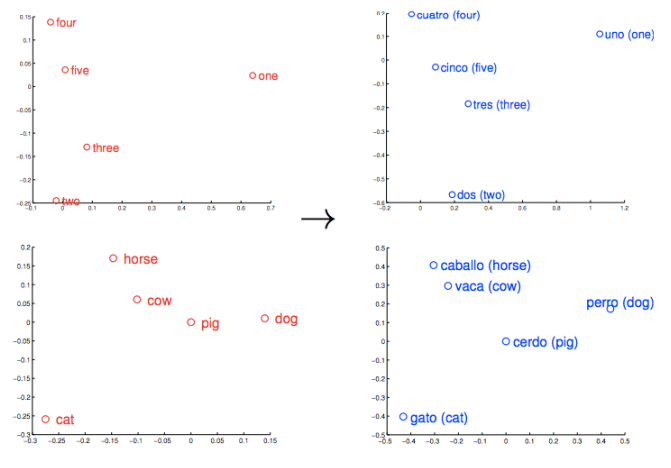
\includegraphics[width=1\linewidth]{word2vec_translation.png}
%	\caption[bla.]{Two examples of distances extracted from word vectors from English and Spanish texts. The top shows the mappings of words of numbers until five and the bottom one of different animals.}
%	\label{fig:w2v}
%\end{figure}
%In Figure \ref{fig:w2v} we can see an example of the similarities between words in different languages. 

In the beginning of our experiments we used \textbf{word2vec} \cite{word2vec}, a special embedding technique for words. Word2vec groups word vectors based on learned semantics. Although word2vec is not trained with any specific language grammar, it is able to make similarities among two languages. Later, we switched to another, similar embedding, see section \ref{sec:model} for further details.

We used keras \cite{keras} for our implementation in python. Keras is a popular neuronal network framework based on Tensorflow \cite{tensorflow}.
\medskip
\section{Proposed Approaches}
\label{sec:model}

For our analysis, we implemented three different approaches to solve the problem of classification. Thus, we compare three different solutions all by using neural architectures. We used Python with Keras backend to train our models. Consisting of a Multi-Layer Perceptron (MLP), a Convolutional Neural Network (CNN) and a long short-time memory (LSTM).

To load the data we use the already built-in Keras function to import the IMDb corpus. The reviews have been already preprocessed and words are indexed to its number of occurrence in the corpus. We set the maximum of words up to $5000$ and a maximum review length to $500$ words. 

For the embedding vector, we also use a built-in Keras function to train it. We specify an output length of $32$, resulting in a $500*32$ embedding vector. The default Keras function works similarly to word2vec. The difference is that with the Keras embedding layer we try to minimize the loss function. On the other hand, word2vec gives an embedding vector that keeps the semantic relation between words. Consequently, the embedding Keras vector might be useful for capturing only polarity of emotions. Nevertheless, the idea still keeps similar for both approaches. 
\medskip
\subsection{Embedding}
As mentioned in section \ref{sec:background}, we used to use the word2vec embedding for our experiments. We implemented a version of it ourselves, trained it and got good results. We later learned about the embedding layer \cite{embedding_stackexchange} of the keras library which transforms all input into a special vector. This layer uses a similar technique as word2vec, see \cite{embedding_example} for a comparison of the two methods. For us, the embedding layer delivered almost the same performance while being easier to use and slightly faster.
\medskip
\subsection{Multi Layer Perceptron}
MLPs \cite{perceptron,mlp} consist of one input layer, one output layer and one or more densely connected layers inbetween. It is one of the most simple existing artificial neural networks. Nonetheless, it is known that works as good as other more complex architectures with simple tasks. MLPs were first designed to make class prediction of a certain data. They need labelled training data to adjust their weights and find decision boundaries between data. It is the most simpler, but powerful, ANN used. Since we are dealing with a binary classification problem, it is a good candidate for having good results using less computational resources than other approaches. In our scenario, we have created an MLP with $250$ fully connected neurons with a rectified linear unit (ReLU) activation function. Detailed visualization of the structure of the model can be seen in Figure \ref{fig:mlp}.

\begin{figure}[tbp!]
	\centering
	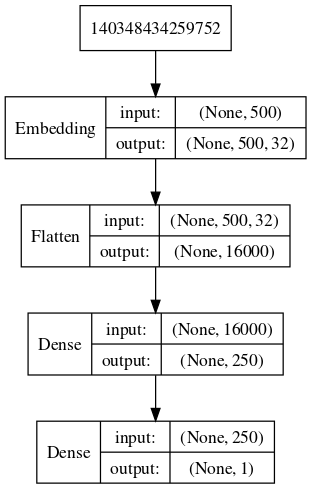
\includegraphics[width=.59\linewidth]{model_MLP.png}
	\caption[bla.]{A detailed structure of the MLP. The embedded vector gets flattened before being send to a fully connected layer. We use binary classification.}
	\label{fig:mlp}
\end{figure}
\newpage
\subsection{Convolutional Neural Network}
Convolutional neural networks (CNNs) \cite{cnn, cnn2} are neural architectures that can learn features from data vectors themselves. They use specialised layers to learn and apply filters to the dataset. CNNs have been proven to overcome many other neural architectures in terms of accuracy, specifically in the vision research field. The typical CNN architecture consists of a convolution layer, where a linear convolution is applied to the input, with a certain kernel size. A max-pooling layer is added to the architecture to reduce the size of the convolution. Moreover, a fully connected layer is appended to get a classification outcome. The convolution and max-pooling layers can be added arbitrarily to the network to get to a certain vector size. It is known that for every convolutional layer it is added, different level of features can be learned. First layers of the network can learn low levels of features and the more you add, higher complexity features. That is why the 'Deep Learning' term is used, to describe a certain network with more than a couple of layers. The shortcoming of deep networks is that the number of weights to tune while training is huge. Therefore, is computationally expensive to train such networks. In our case, we only add one time the convolutional layer. We expect to learn basic features about the data. Therefore, in Figure \ref{fig:cnn} we can see how our architecture looks like.  We use $32$ filters and a $3*3$ kernel size for the convolution layer. The activation function is again ReLU. For the max-pooling layer, we reduce our size by a factor of $2$. Then we add a fully connected layer of $250$ neurons along with the last binary classification.

\begin{figure}[tbh!]
	\centering
	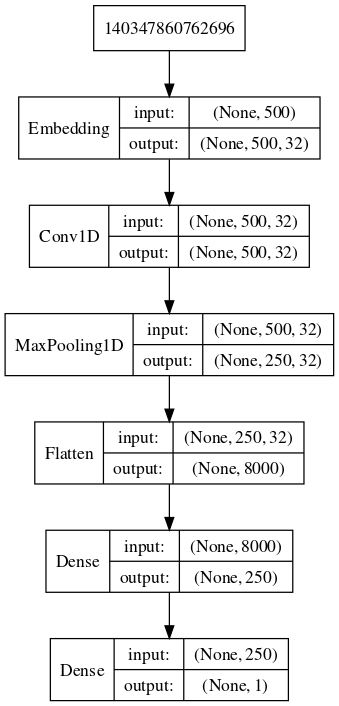
\includegraphics[width=.59\linewidth]{model_CNN.png}
	\caption[bla.]{The CNN model. The special features are the convolutional layer and the sub-sampling layer that reduces our feature space. The subsequent part is equal to the MLP.}
	\label{fig:cnn}
\end{figure}
\newpage
\subsection{Long Short-Time Memory Network}
LSTM networks \cite{lstm} are a type of recurrent neural network (RNN) which are used a lot in the natural language processing field and other fields working with time dependant data. They can learn more long-term dependencies than a simple RNN. Since we are working with texts that are longer than a sentence, LSTM is also a good candidate. In Figure \ref{fig:lstm} we can see a detailed explanation of the architecture used. We use $n=100$ as the dimensionality of the output space. \\

\begin{figure}[bp!]
	\centering
	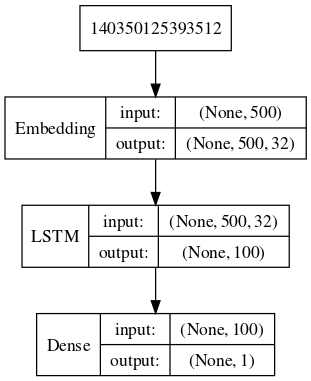
\includegraphics[width=.59\linewidth]{model_LSTM.png}
	\caption[bla.]{Structure of the used LSTM architecture. In keras exists a LSTM layer which abstracts from the common gates and structures of a LSTM for easier implementation.}
	\label{fig:lstm}
\end{figure}
\newpage
\subsection{Short Discussion of the used Architectures}
In each of the above models, we need to add a last layer into the network. The output layer is responsible for classifying between negative and positive reviews and thus consists of only one neuron. The loss function of our models is the binary cross entropy and we are especially interested in the accuracy of the trained model. 

We used the three introduced architectures because of their popularity and their diverse properties. All three belong to the most used types of neural networks \cite{neural_networks_overview}. The MLP is supposed to give a baseline for the reults of the other networks. With the CNN, we tried to overcome the literal nuances problem. We believed that by using this self-learning feature approach such complexities could be overcame. By using hte LSTM cells, we tried to leverage the fact that language is time dependent. It is clear that a word has several relation to its precedent and future words. With the three different architectures we have benefitts and drawbacks for using them, therefore is worth try them three. Moreover, all networks achieved acceptable results.

\section{Results}
\label{sec:results}
We achieved similar results with all three different neural networks. The MLP and CNN both took between ten and fifteen minutes to train on a single CPU and the LSTM over two hours. Given the absence of big differences in the prediction accuracy, training the LSTM is not really worth it. Our best performing network is the presented CNN structure, trained for just one epoch, with a prediction accuracy of 87.80\% on the test set. In the Kaggle challenge \cite{Kaggle} would have placed 267th out of the 578 participants which is above average and better than the three baseline classifiers \cite{kaggle_baselines} for this competition. In table \ref{tab:resu}, we can find a described numeric values for the results for the presented architectures. 

\begin{table}[tbh]
\begin{center}
	\begin{tabular}{ | c | c | c | c | } 
		\hline
		&\textbf{MLP} & \textbf{CNN} & \textbf{LSTM} \\ 
		\hline
		1 epoch & 87.33 & 87.80 & 84.67 \\
		\hline
		10 epochs & 86.16 & 87.59 & 86.29 \\
		\hline
	\end{tabular}
	\caption{Accuracy on the test set of the different architectures after one and after ten epochs.}
	\label{tab:resu}
\end{center}
\end{table}

Detailed plots of the train and test loss and accuracy can be found in the appendix. It is clear that after the first training epoch, the test accuracy stays about the same, just the training accuracy increases. Training for more than one epoch does not bring any merit. We can spot some overfitting because the test loss increases as the test accuracy stays the same. The network makes wrong decisions while being more sure about it. This could mean that the networks are bigger than needed for the task. Dropout could be used to circumvent this as well as a smaller batch size and smaller learning rate.
%It is surprising that the three different network architectures' accuracy was so alike. Even the loss across the epochs seems to be almost the same for all networks, aswell as the training accuracy. 
\section{Conclusion}
\label{sec:concl}

On the given dataset, acceptable results can be achieved with a variety of different methods. Capturing time-related dependencies (as a LSTM does) or learning filters (as a CNN does) does not seem to add a lot of performance for this specific use case. But it could also be either the task, the dataset or even the preprocessing and embedding that diminishes the variety of our results. 

Our experiements show that for certain machine learning tasks, there can be several different approaches which despite structural differences manage to perform similar. In such a case, it is advisable in regard of overall efficiency to choose a network that is easier or faster to train, like the MLP or CNN in our experiments. It is plausible that further optimizations and tweaking of the hyperparamters would lead to more apparent differences between the networks and other performance characteristics.

% insert your bibliographic references into the bib.bib file
%\bibliographystyle{plain}
%\addcontentsline{toc}{section}{Bibliography}% Add to the TOC
\bibliographystyle{unsrt}
\bibliography{kpis_bib}

\begin{figure*}[tbh!]
	\centering
	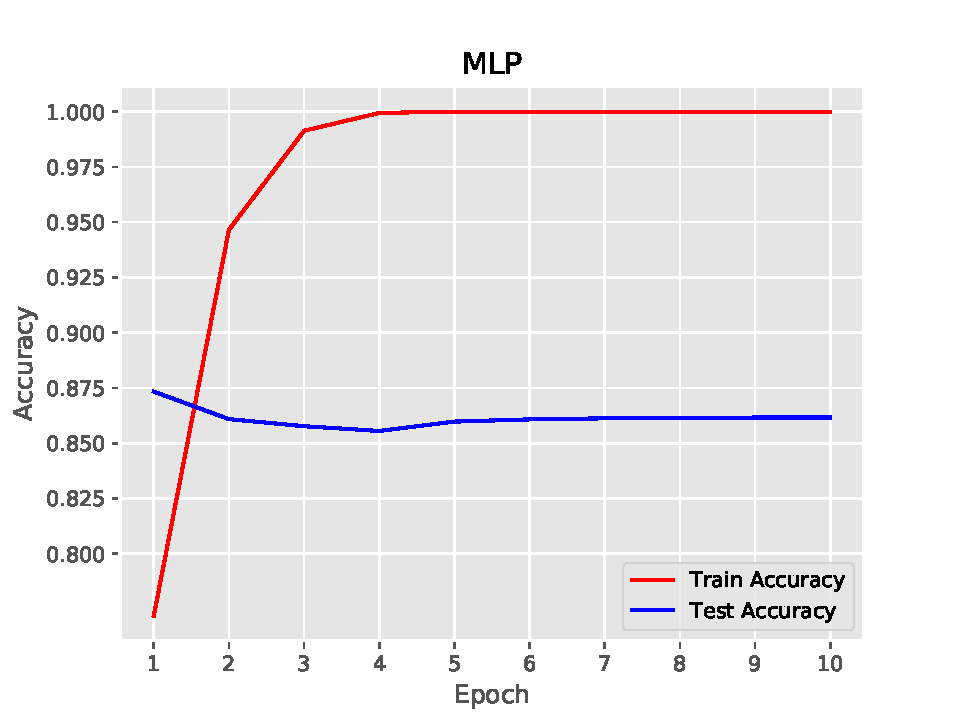
\includegraphics[width=.7\linewidth]{../mlp-acc_10epochs.pdf}
	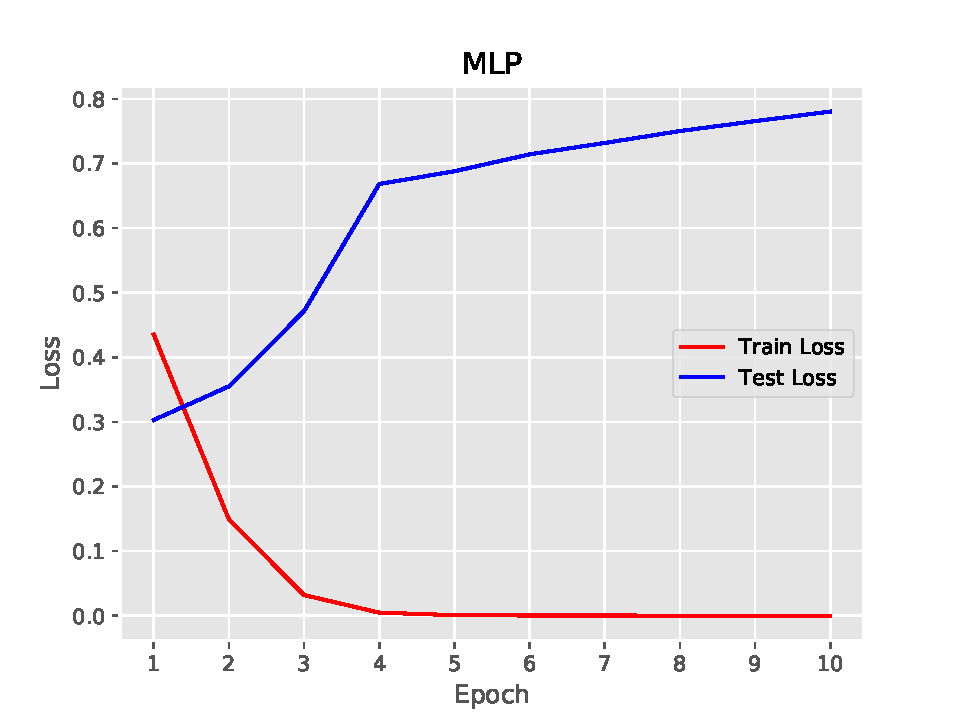
\includegraphics[width=.7\linewidth]{../mlp-loss_10epochs.pdf}
	\caption{MLP accuracy and loss.}
\end{figure*}
\begin{figure*}
	\centering
	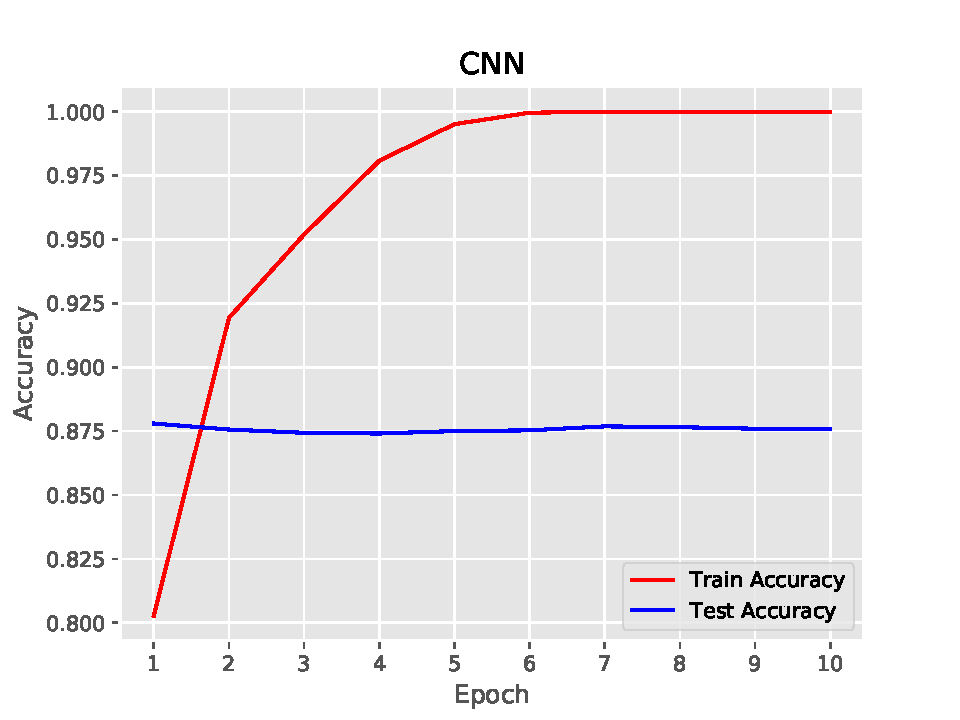
\includegraphics[width=.7\linewidth]{../cnn-acc_10epochs.pdf}
	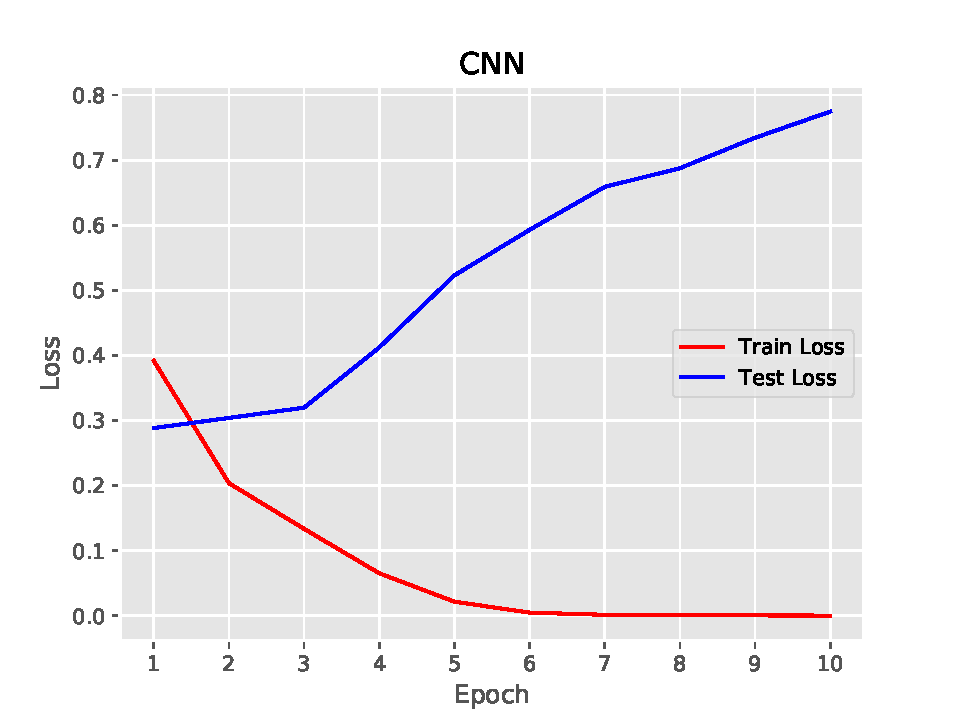
\includegraphics[width=.7\linewidth]{../cnn-loss_10epochs.pdf}
		\caption{CNN accuracy and loss.}
\end{figure*}
\begin{figure*}
	\centering
		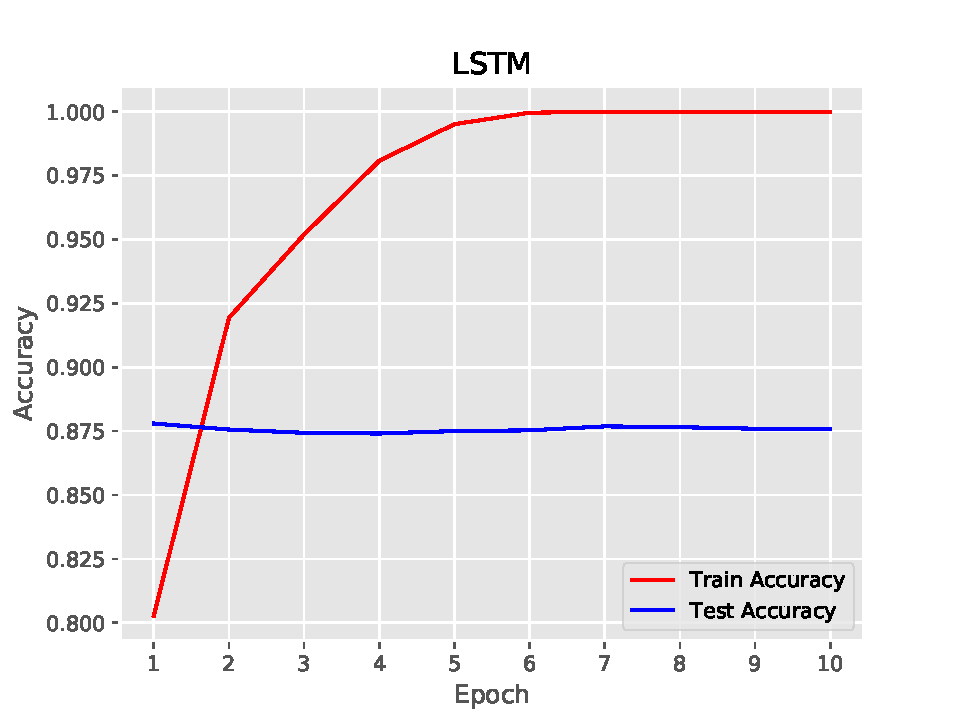
\includegraphics[width=.7\linewidth]{../lstm-acc_10epochs.pdf}
	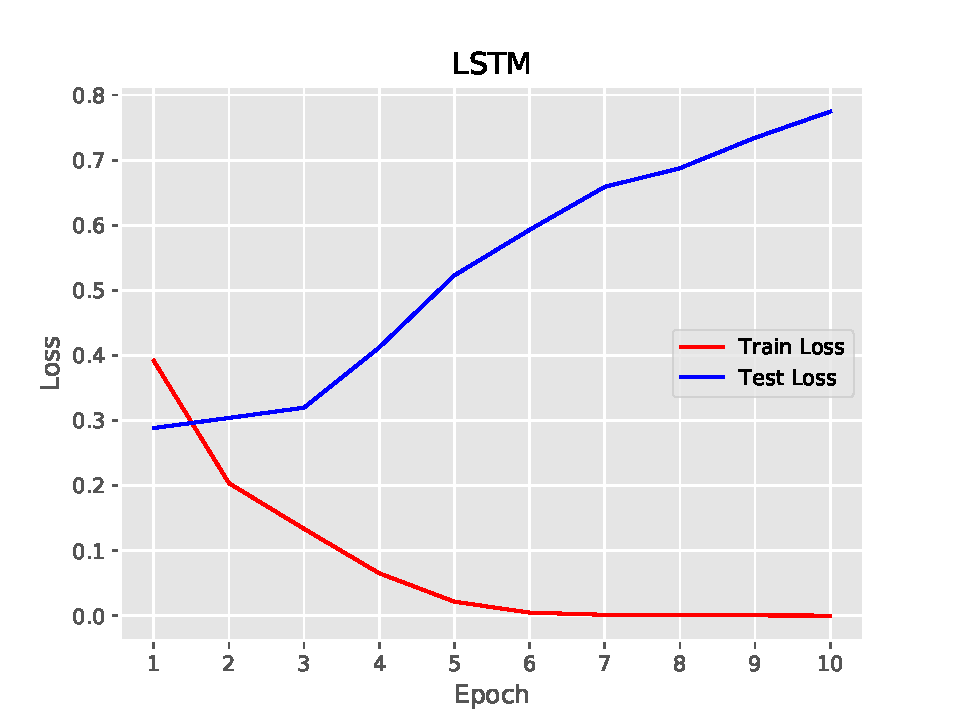
\includegraphics[width=.7\linewidth]{../lstm-loss_10epochs.pdf}
	\caption{LSTM accuracy and loss.}
\end{figure*}




%\bibliography{kpis_bib}
\end{document}
